\documentclass[tikz,border=14pt]{standalone}
\usepackage{amsmath,amssymb}
\usetikzlibrary{arrows.meta}
\definecolor{ink}{HTML}{E4EDF8}
\definecolor{muted}{HTML}{596B80}
\definecolor{blue}{HTML}{9FC2FF}
\definecolor{teal}{HTML}{63D3BB}
\definecolor{gold}{HTML}{E7C274}
\definecolor{panel}{HTML}{111923}
\pagecolor{panel}
\color{ink}
\begin{document}
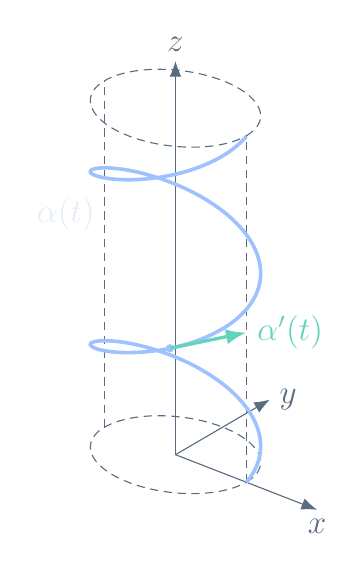
\begin{tikzpicture}[font=\large,text=ink,x={(.9cm,-.35cm)},y={(.6cm,.35cm)},z={(0cm,1cm)},vec/.style={-{Latex[length=2.6mm]},line width=1.2pt},axis/.style={muted,-{Latex[length=2mm]},thin}]

\draw[axis] (0,0,0)--(2,0,0) node[below] {$x$};
\draw[axis] (0,0,0)--(0,2,0) node[right] {$y$};
\draw[axis] (0,0,0)--(0,0,5) node[above] {$z$};
\foreach \h in {0,4.4} {\draw[muted,densely dashed] plot[domain=0:360,samples=70] ({cos(\x)},{sin(\x)},\h);}
\draw[muted,densely dashed] (1,0,0)--(1,0,4.4);
\draw[muted,densely dashed] (-1,0,0)--(-1,0,4.4);
\draw[blue,line width=1.3pt] plot[domain=0:720,samples=200] ({cos(\x)},{sin(\x)},{\x/164});
\coordinate (P) at ({cos(300)},{sin(300)},{300/164});
\fill[blue] (P) circle(1.5pt);
\draw[vec,teal] (P)--++({-.9*sin(300)},{.9*cos(300)},.315) node[right] {$\alpha'(t)$};
\node[left] at (-1,0,2.7) {$\alpha(t)$};

\end{tikzpicture}
\end{document}
